\section{Part: Statistics and parameter estimation }\label{sec:q1}    

\subsection{}

\indent In order to check for linearity of the least squares method, that needs to be applied, 
\begin{center}
	$\bar{y} = A (\bar{x}) + \bar{\epsilon}$
\end{center}
design matrix $A$ has to be derived. The curve that is being fitted is given by
\begin{center}
	$r = \sqrt{(x-x_0)^2+(y-y_0)^2}
\end{center}
Therefore, the LSM equation is
\begin{figure}[H]
		\centering
		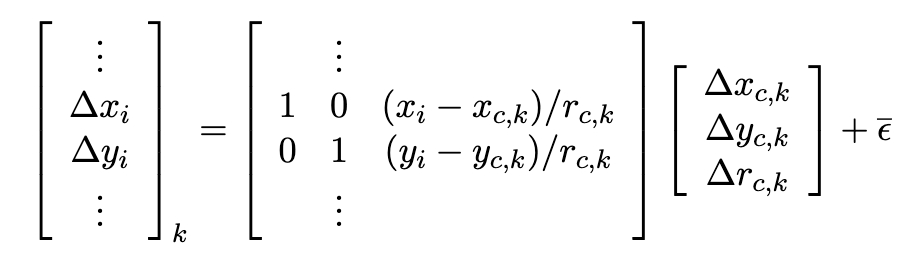
\includegraphics[width=0.4\linewidth]{eq1.png}
\end{figure}
As it can be observed, the design matrix is dependent on estimated parameters $\bar{x}$. This means it is a non-linear problem, which needs to be solved iteratively. 

\subsection{}

\indent Given $Q_{yy} = P_{yy} = \lambda I$, the estimated parameters and their covariances might be found by applying
\begin{figure}[H]
		\centering
		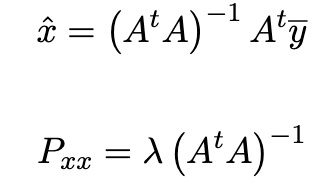
\includegraphics[width=0.2\linewidth]{eq2.png}
\end{figure}
which proves that $\hat{x}$ is independent of $\lambda$, whereas its covariance matrix $P_{xx}$ indeed is a function of $\lambda$.

\subsection{}
The problem statement was presented in class. Below, relevant equations are given. 
\begin{figure}[H]
		\centering
		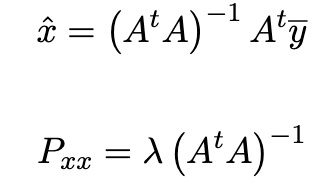
\includegraphics[width=0.2\linewidth]{eq2.png}
\end{figure}
This set of equations describes 3-dimensional rotation (by three rotation matrices R) and translation (by vector b) of the point clouds in order to fit them together. Linearization is done by taking partial derivatives of the observation equation w.r.t. three angles, which are parameters to be estimated in this case.



\subsection{}
i) Finding eigenvalues and eigenvectors of the problem enables statement, whether there is a solution of manifolds or a unique solution. Manifold of solutions occur for rank-deficient systems (for which one or more eigenvalues are null).\\
ii) Yes, the model based on two sets of observations is rank-deficient and will therefore result in a manifold of solutions. This property is manifested by multiple different interpretations of the comet geometry. 


    
